\documentclass{article}
\usepackage[UTF8]{ctex}
\usepackage{pythonhighlight}
\usepackage{listings}
\lstset{
    basicstyle          =   \tt,          % 基本代码风格
    identifierstyle=\color{brown!80!black},
    keywordstyle        =   \color{purple}\bfseries,          % 关键字风格
    commentstyle        =   \rmfamily\itshape,  % 注释的风格,斜体
    stringstyle         =   \ttfamily,  % 字符串风格
    flexiblecolumns,                % 别问为什么,加上这个
    numbers             =   left,   % 行号的位置在左边
    showspaces          =   false,  % 是否显示空格,显示了有点乱,所以不现实了
    numberstyle         =   \zihao{-5}\ttfamily,    % 行号的样式,小五号,tt等宽字体
    showstringspaces    =   false,
    captionpos          =   t,      % 这段代码的名字所呈现的位置,t指的是top上面
    frame               =   lrtb,   % 显示边框
    backgroundcolor=\color[RGB]{245,245,244},
}
% Language setting
% Replace `english' with e.g. `spanish' to change the document language
\usepackage[english]{babel}
\usepackage{float}
% Set page size and margins
% Replace `letterpaper' with `a4paper' for UK/EU standard size
\usepackage[letterpaper,top=2cm,bottom=2cm,left=3cm,right=3cm,marginparwidth=1.75cm]{geometry}

% Useful packages
\usepackage{amsmath}
\usepackage{graphicx}
\usepackage[colorlinks=true, allcolors=blue]{hyperref}

\title{数逻实验报告Lab5}
\author{雷远航}

\begin{document}

\maketitle

\begin{abstract}
实验项目:变量译码器
\end{abstract}

\section{操作方法与实验步骤}

\subsection{原理图设计实现74LSLS138译码器模块}

\subsubsection{画出原理图}
用原理图的方式在ISE中绘制译码器
    \begin{figure}[H]
	\centering
	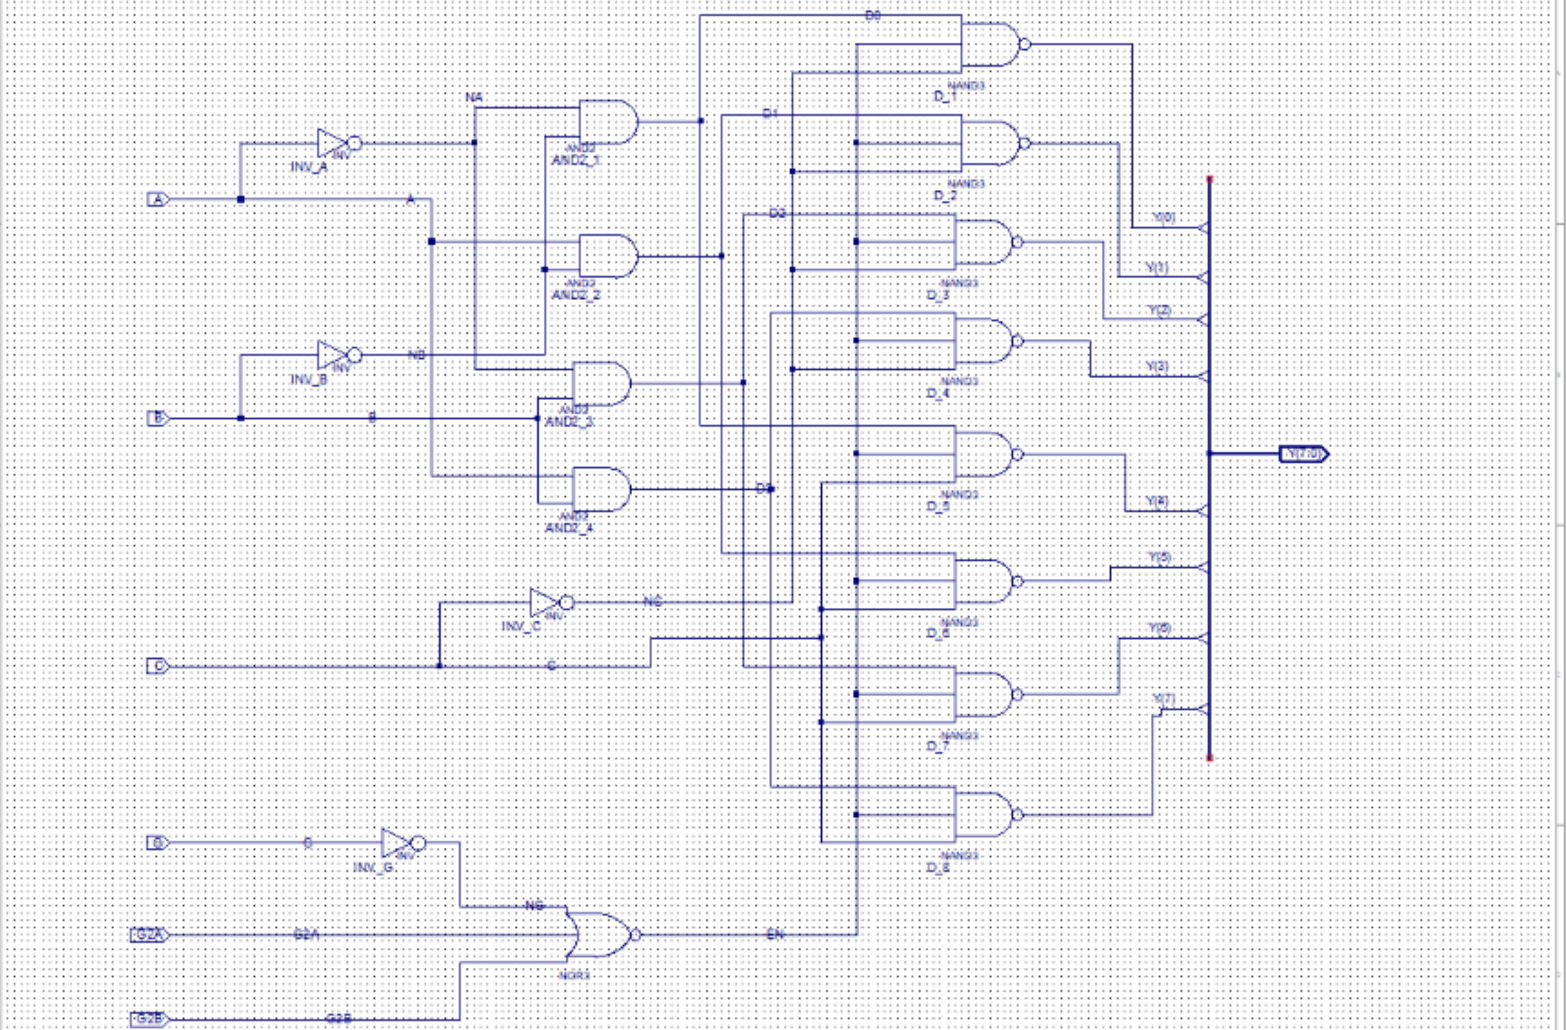
\includegraphics[width=0.7\textwidth]{9.png}
	\caption{\label{Lab5}原理图}
	\end{figure}

\subsubsection{在ISE中运行生成HDL代码}
Check Design Rules检查错误,运行Synthesize,使用View HDL Function Model查看HDL代码
    \begin{figure}[H]
	\centering
	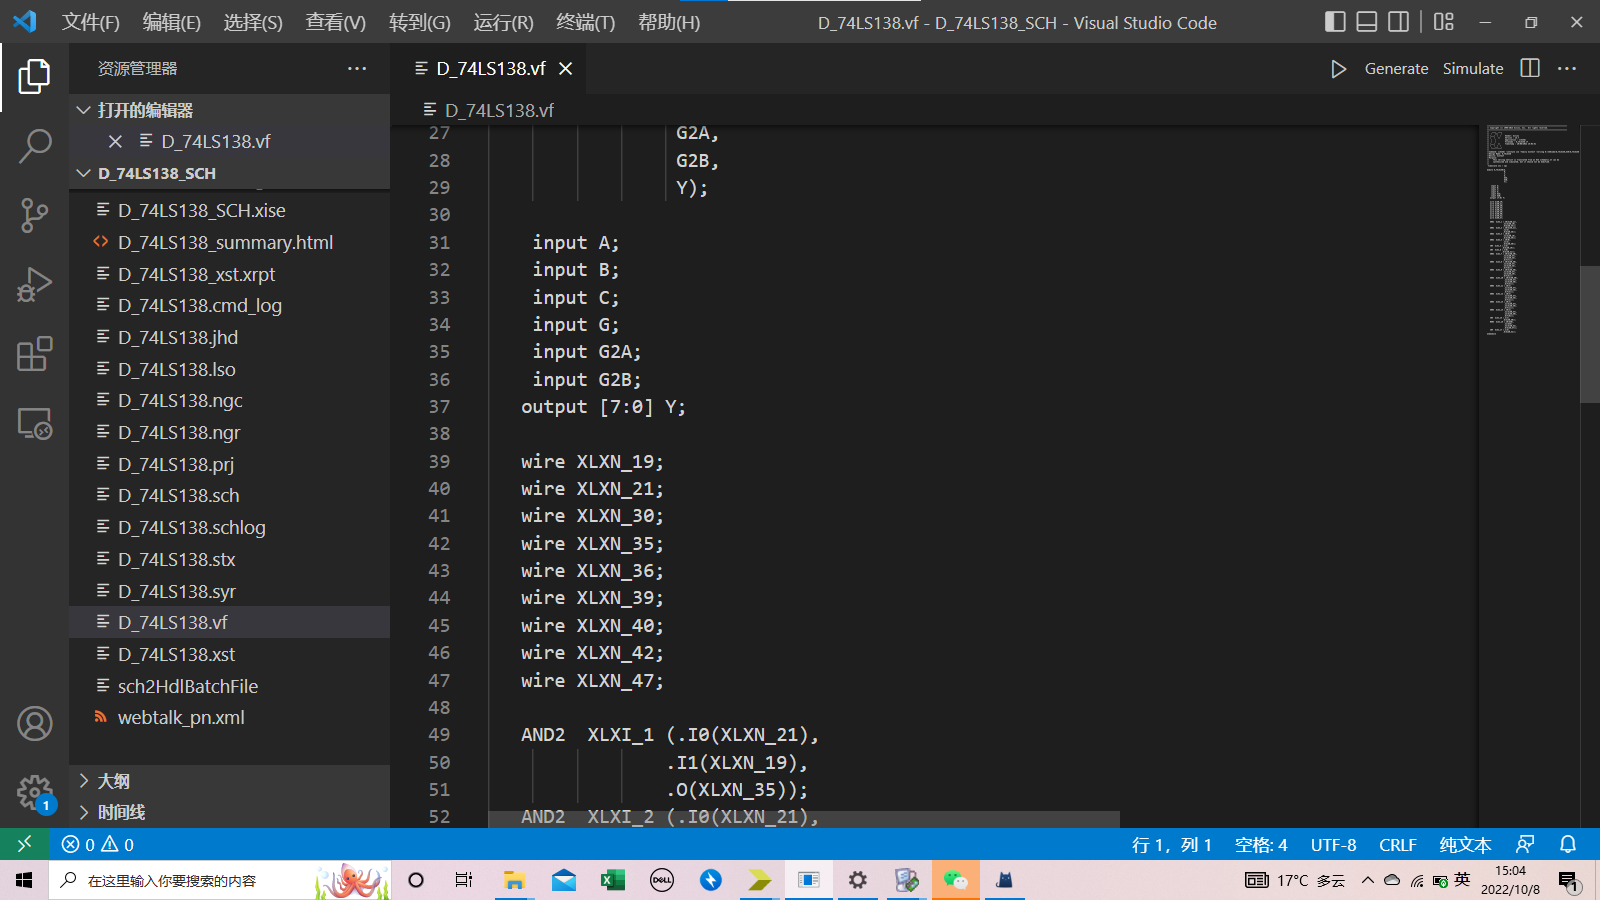
\includegraphics[width=0.6\textwidth]{2.png}
	\caption{\label{Lab5}HDL}
	\end{figure}

\subsubsection{对模块进行仿真}
    导入测试文件对模块进行模拟仿真
\begin{lstlisting}[language=verilog]
	`timescale 1ns / 1ps
	
	module MyMC14495_tb();
		
	// Inputs
		reg D0;
		reg D1;
		reg D2;
		reg D3;
		reg LE;
		reg point;
		
	// Output
		wire p;
		wire a;
		wire b;
		wire c;
		wire d;
		wire e;
		wire f;
		wire g;
		
	// Instantiate the UUT
		MyMC14495_HDL UUT (
		.D0(D0), 
		.D1(D1), 
		.D2(D2), 
		.D3(D3), 
		.LE(LE), 
		.point(point), 
		.p(p), 
		.a(a), 
		.b(b), 
		.c(c), 
		.d(d), 
		.e(e), 
		.f(f), 
		.g(g)
		);
	// Initialize Inputs
		integer i;
		initial begin
		//$dumpfile("MyMC14495_HDL.vcd");
		//$dumpvars(1, MyMC14495_HDL_tb);
		
		D3 = 0;
		D2 = 0;
		D1 = 0;
		D0 = 0;
		LE = 1'b0;
		point = 0;
			
		for (i=0; i<=15; i=i+1) begin
			{D3,D2,D1,D0}=i;
			point = i;
			#50;
		end
			  
		#50;
		LE = 1'b1;
		#10;
		end
	endmodule
		
\end{lstlisting}
测试代码解释:

1.测试时的输入部分为六个寄存器(reg):G,G2A,G2B,C,A,B.他们与所画原理图的输入部分相对应

2.输出部分为8位的网线(wire)Y

3.实例化自己所画的模块D 74LS138,命名为UUT

4.在inital部分中对输入部分的值进行相应的改变和赋值,从而达到测试的目的

在本initial块中,设置G,G2A和G2B确保总控为开启的状态,然后通过for 语句遍历可以改变A,B,C的输入从而可以在波形图上显示




\subsubsection{完成全部操作}
    
\begin{figure}[H]
	\centering
	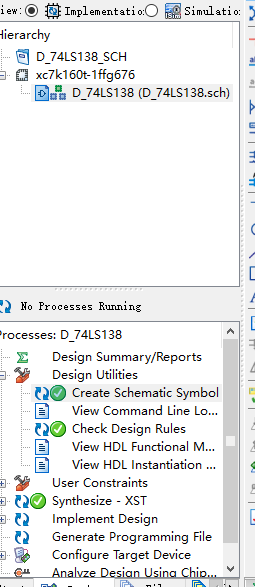
\includegraphics[width=0.2\textwidth]{4.png}
	\caption{\label{Lab5}验证}
	\end{figure}


%\subsection{a}
\subsection{验证D 74LS138}

\subsubsection{D 74LS138 TEST原理图}

导入第一个工程的 *.sym 与 *.vf 到第二个工程当中,进行原理图的绘制
    \begin{figure}[H]
	\centering
	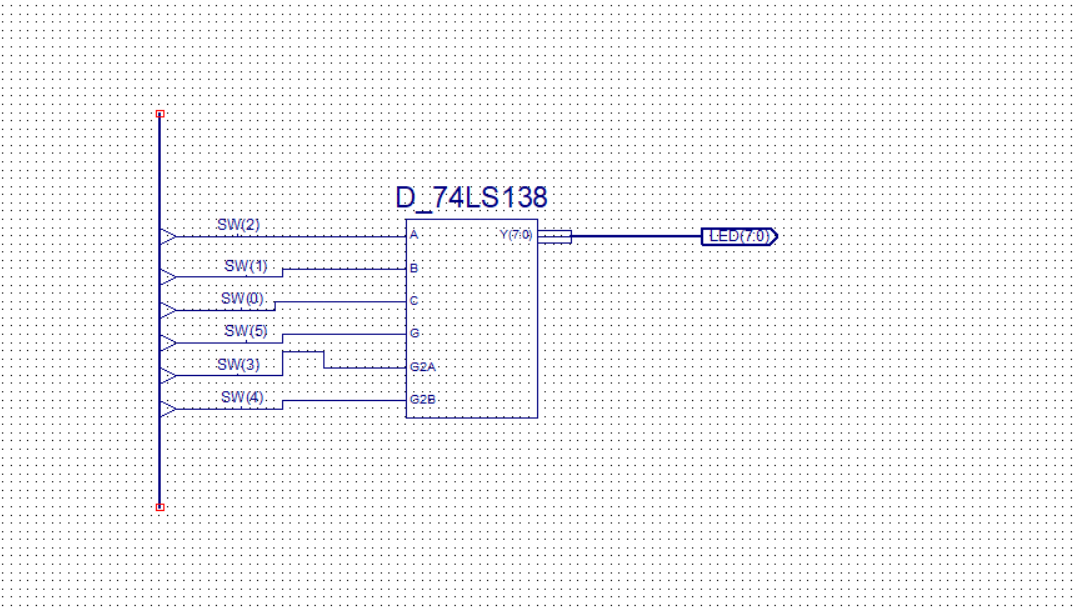
\includegraphics[width=0.7\textwidth]{5.png}
	\caption{\label{Lab5}原理图}
	\end{figure}

\subsubsection{下版验证}
导入SWORD4.ucf文件,将生成的.bit文件导入到实验版中,进行实验结果的验证


\subsection{实现楼道灯控制}

\subsubsection{进行原理图绘制}
导入第一个工程的 *.sym 与 *.vf 到第三个工程当中,进行原理图的绘制
    \begin{figure}[H]
	\centering
	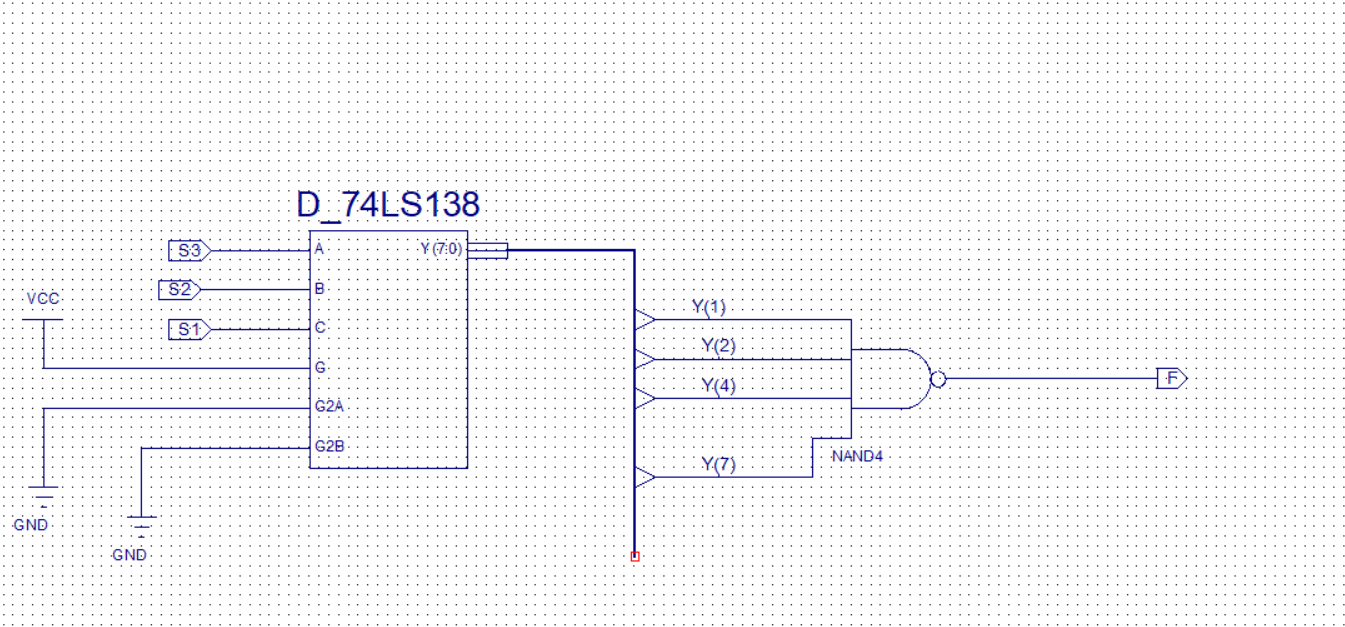
\includegraphics[width=0.7\textwidth]{7.png}
	\caption{\label{Lab5}原理图}
	\end{figure}

\subsubsection{对模块进行模拟仿真}
导入仿真激励代码,进行模拟仿真

测试文件各部分的意义已在1.1.3节中进行说明.

\subsubsection{下版验证}

导入SWORD4.ucf文件,将生成的.bit文件导入到实验版中,进行实验结果的验证


\subsection{Bonous:LampCtl.v的验证}

\subsubsection{自行书写LampCtrl.v}
\begin{lstlisting}[language=verilog]
	module Decoder(
		input wire S1,
		input wire S2,
		input wire S3,
		output wire K1,
		output wire K2
	);
	
	reg [2:0] test;
	reg temp1;
	reg temp2;
	
	always @(*) begin
	
	
	test = {S3,S2,S1};
	temp1 = 1'b0;
	temp2 = 1'b0;
	
	case (test) 
	
	3'b001:temp1 = 1'b1;
	3'b111:temp2 = 1'b1;
	
	
	
	endcase
	
	end
	assign K1 = temp1;
	assign K2 = temp2;
	 
	endmodule
	
	module OR(
		input wire S1,
		input wire S2,
		output wire F
	);
	
	assign F = S1|S2;
	
	endmodule
	
	module LampCtrl(
		input wire S1, 
		input wire S2, 
		input wire S3,
		output wire F
		);
		wire K1;
		wire K2;
		Decoder d1(S1,S2,S3,K1,K2);
		OR d2(K1,K2,F);
	
		
	
	endmodule 
\end{lstlisting}
\subsubsection*{代码解释}
在Decoder模块中传入三个开关的信号S1,S2,S3,以及灯是否闪亮的两种情况的结果K1,K2.
当结果输入的情况为001和111的两种情况时,将对应的输出置为1.

在OR模块中返回两个输入信号取或运算的结果

在LampCtrl模块中,首先调用Decoder模块判断对应的输入情况,然后调用OR模块获得输出的结果

\subsubsection{对代码进行模拟仿真}
\begin{figure}[H]
	\centering
	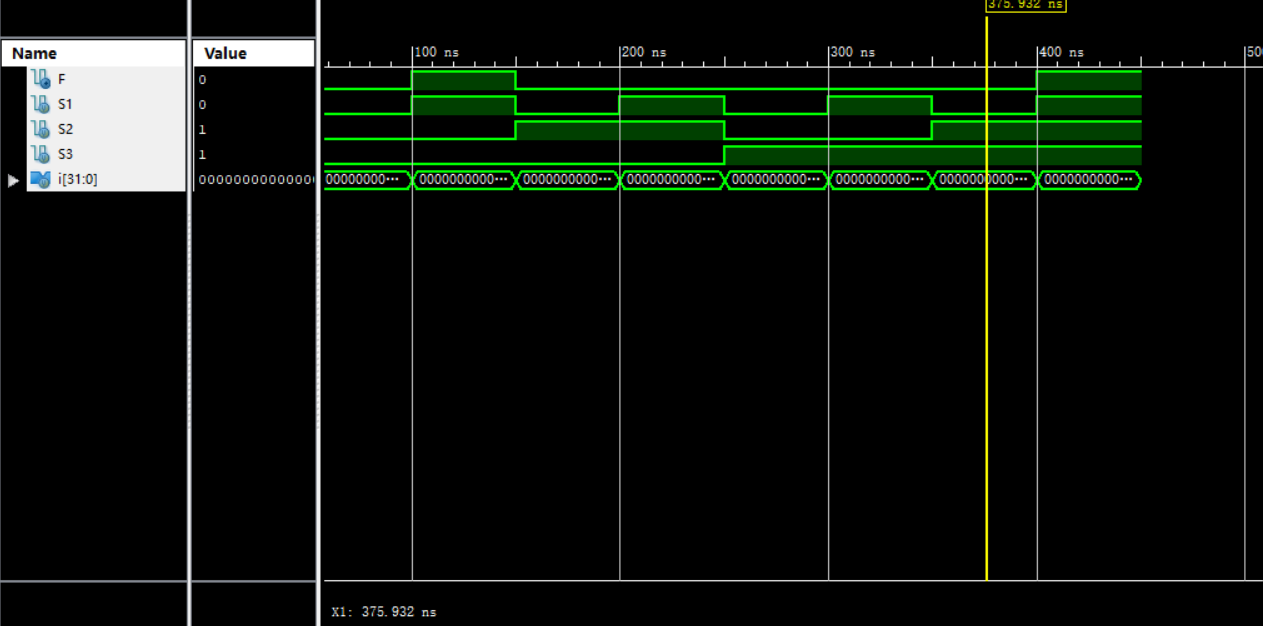
\includegraphics[width=0.7\textwidth]{23.png}
	\caption{\label{Lab5}模拟仿真}
	\end{figure}
\subsubsection*{波形图分析}
在仿真激励代码中,输入{S3,S2,S1},一次从0到7进行赋值,可以发现,当输入为001和111的两种情况时,最终的结果才会输出为1,与所书写的代码的情况符合

\subsubsection*{下版验证}
下版验证时可以看到,当拨动开关的情况为上述所说的两种情况时灯才会闪亮,其他情况并不闪亮.
Bonous部分下版验证已通过验收,因此不再插入图片.

\section{实验结果描述与分析}

\subsection{Part1:译码器原理图验证}

所得到的波形图结果如下:
	\begin{figure}[H]
	\centering
	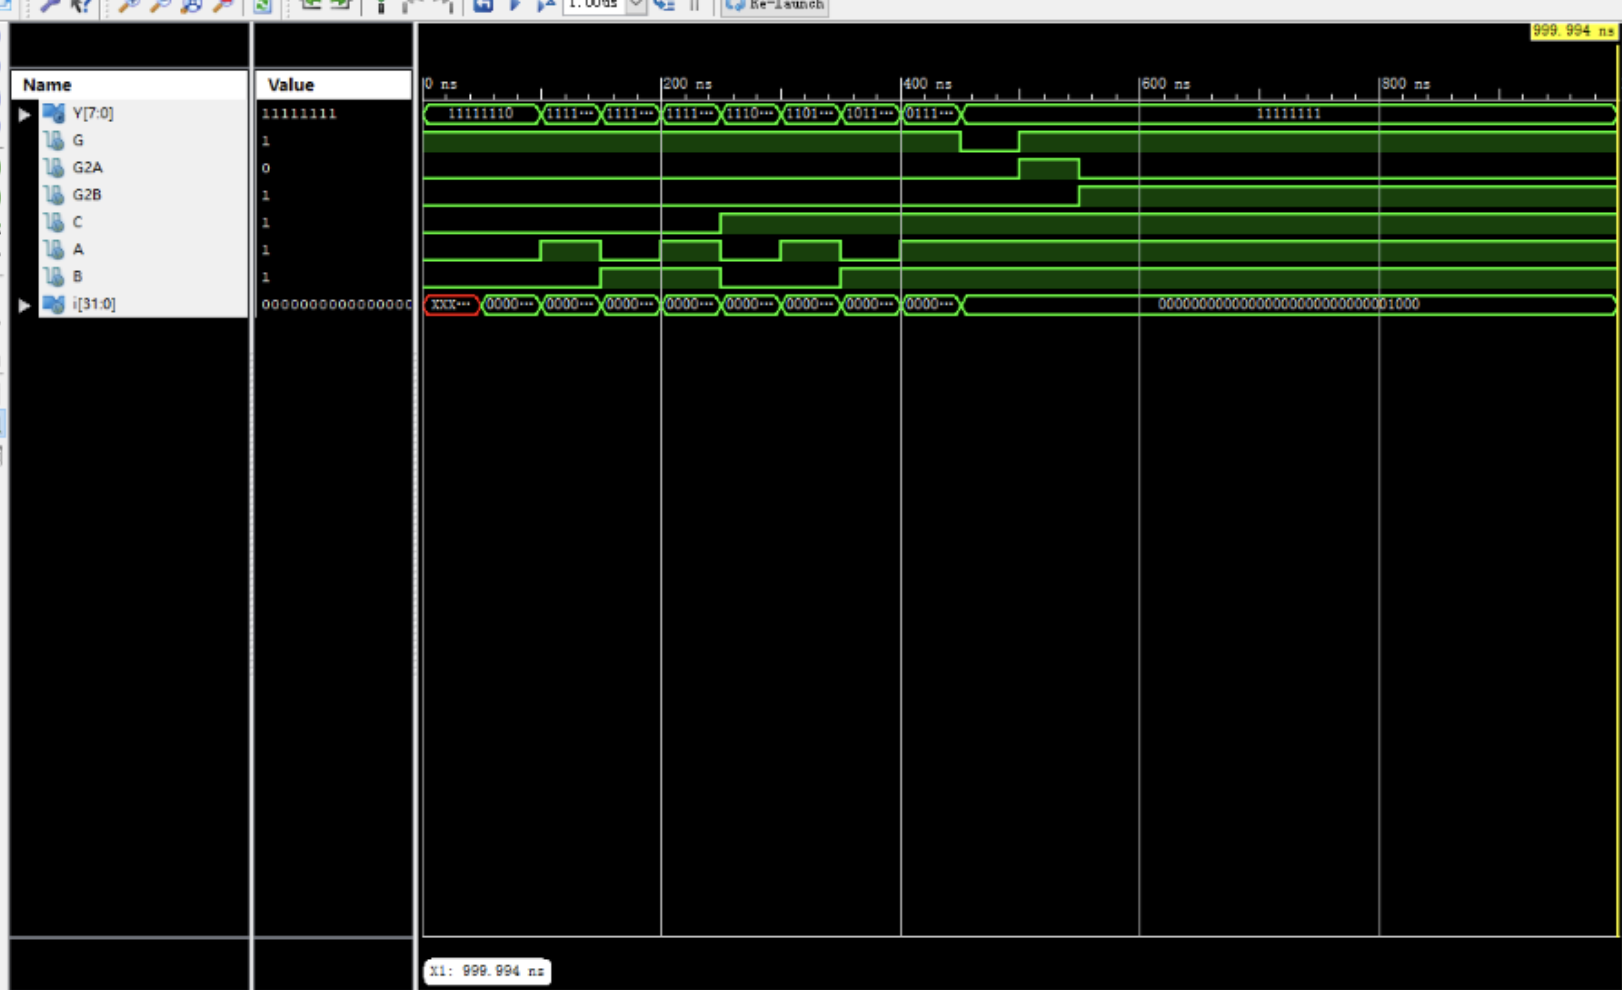
\includegraphics[width=0.7\textwidth]{10.png}
	\caption{\label{Lab5}原理图}
	\end{figure}

\subsection*{波形分析:}

根据测试文件,开始的部分总控为开启状态,所输入的{C,B,A}依次从0到7进行遍历,因此对应的输出为遍历到的倒数第i个位置为0,其余位为1

而后总控开关的状态为关闭,因此输出的所有位都为1



\subsection{Part2:译码器下版验证}

下版验证的结果如下:
	\begin{figure}[H]
	\centering
	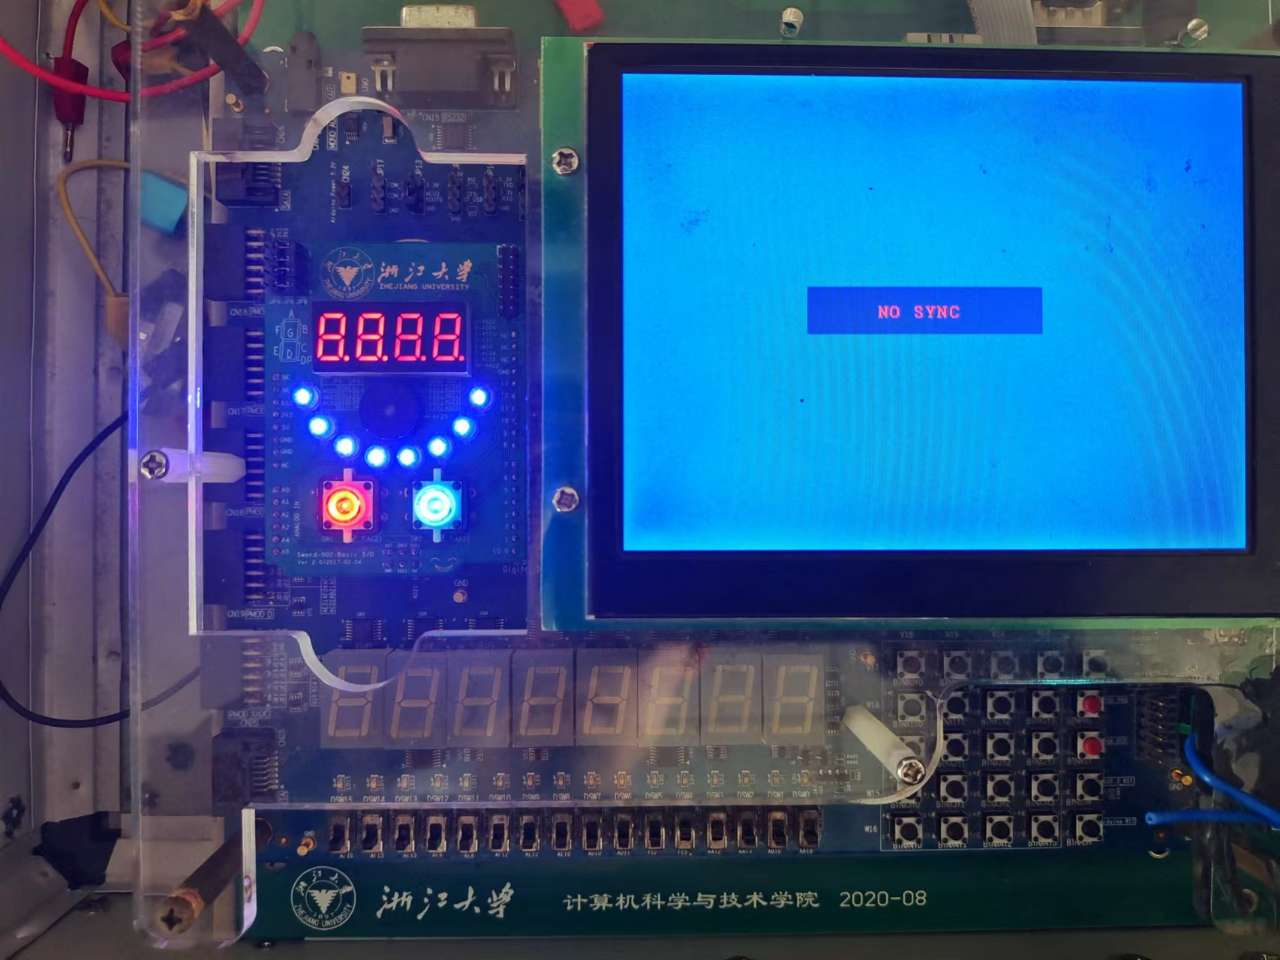
\includegraphics[width=0.5\textwidth]{11.jpg}
	\caption{\label{Lab5}下版验证}
	\end{figure}


	\begin{figure}[H]
	\centering
	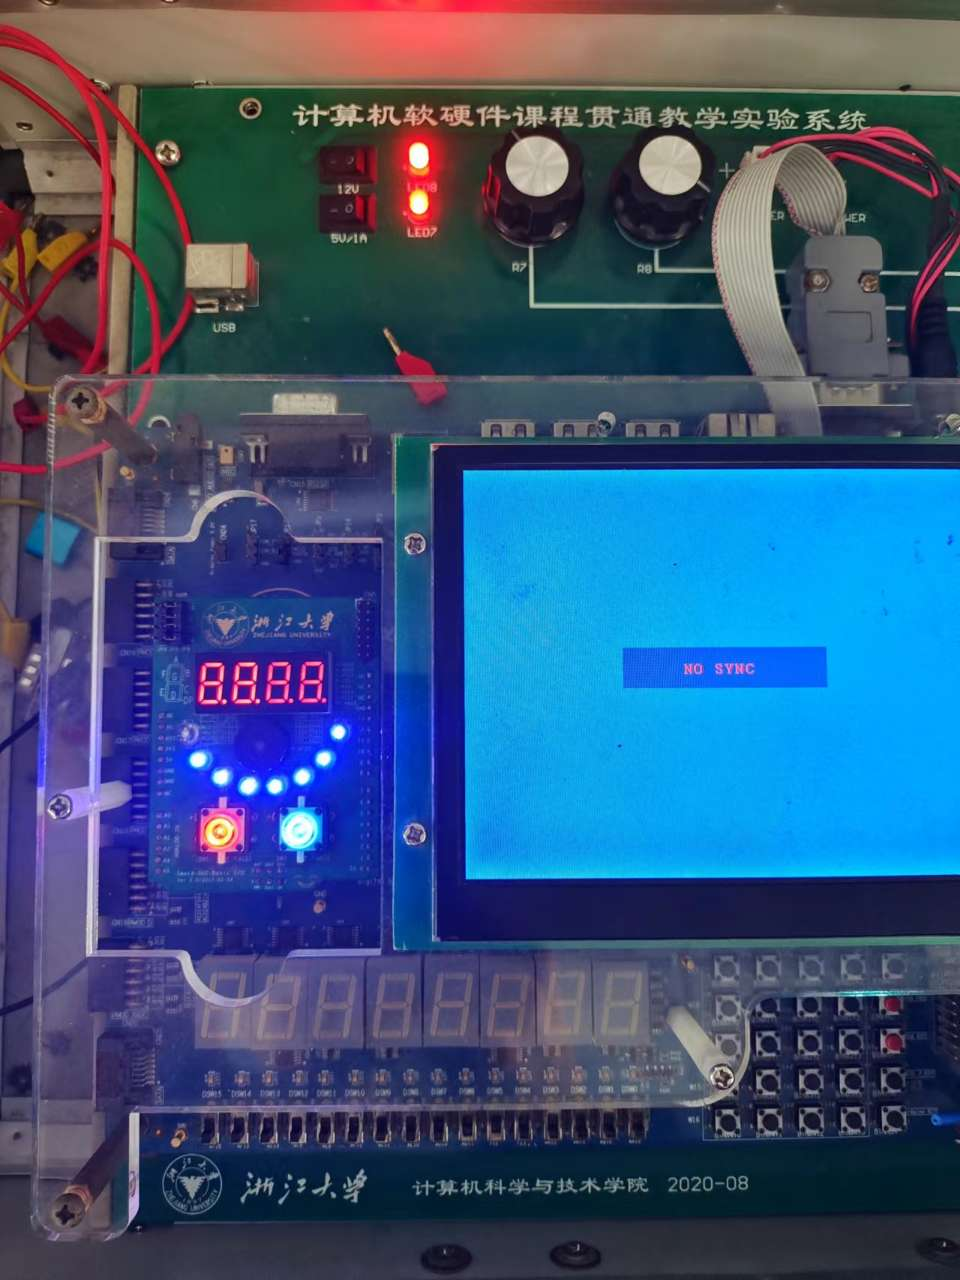
\includegraphics[width=0.5\textwidth]{12.jpg}
	\caption{\label{Lab5}下版验证}

	\end{figure}
	\begin{figure}[H]
	\centering
	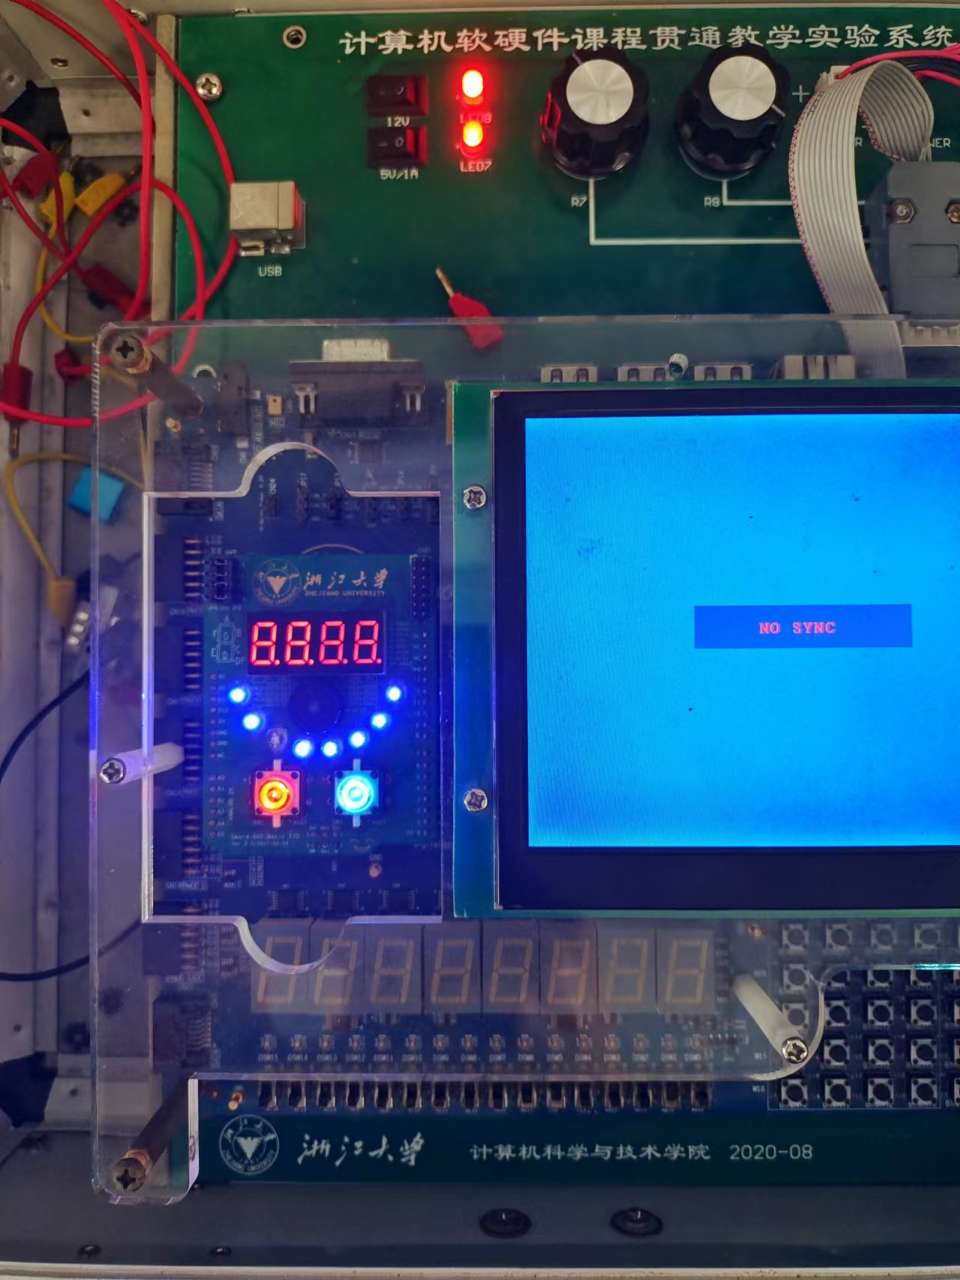
\includegraphics[width=0.5\textwidth]{13.jpg}
	\caption{\label{Lab5}下版验证}
	\end{figure}

\subsubsection*{下版结果解释:}

若控制总控(enable)的三个开关调整为关闭的状态时,如第一张图所示,无论后面的开关如何进行改变所有的灯都处于
闪亮的状态,如果总控的状态调整为开启的状态,那么通过A,B,C输入所绑定的实验版开关输入对应的数字(二进制),对应的第i盏
灯就会熄灭

\subsection{Part3:灯光控制验证}

\subsubsection{波形图}

	
	\begin{figure}[H]
	\centering
	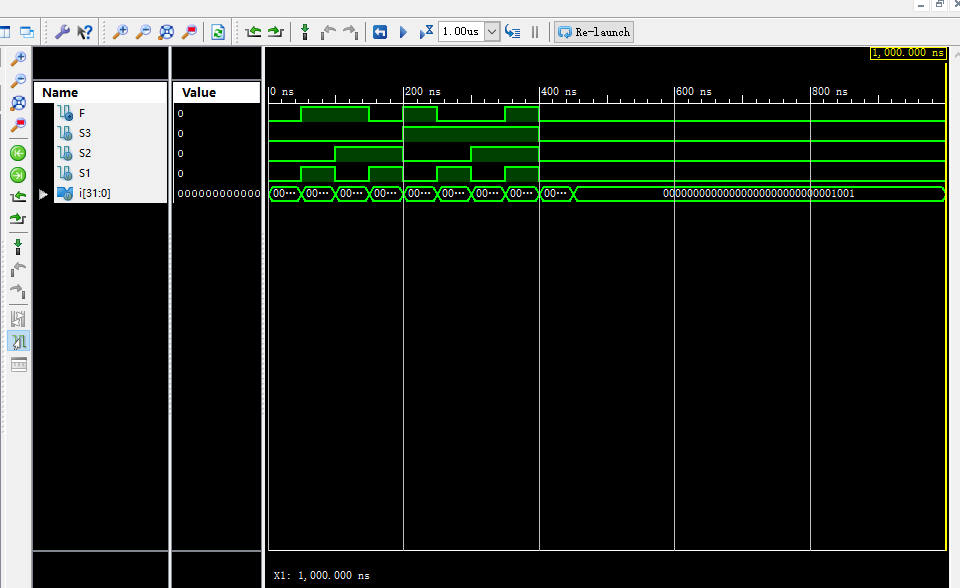
\includegraphics[width=0.7\textwidth]{8.png}
	\caption{\label{Lab5}波形图}
	\end{figure}

波形解释:
	由测试文件可以,对应的输入从0到7遍历,在波形图所示的八个对应段中
	如果有奇数个输入为1时,那么灯光闪亮,对应的输出F为1,通过波形图可以看出
	当输入为\{1,1,1\},\{1,0,0\},\{0,1,0\},\{0,0,1\}时,对应的输出F为1


\subsubsection{下版验证}

	\begin{figure}[H]
	\centering
	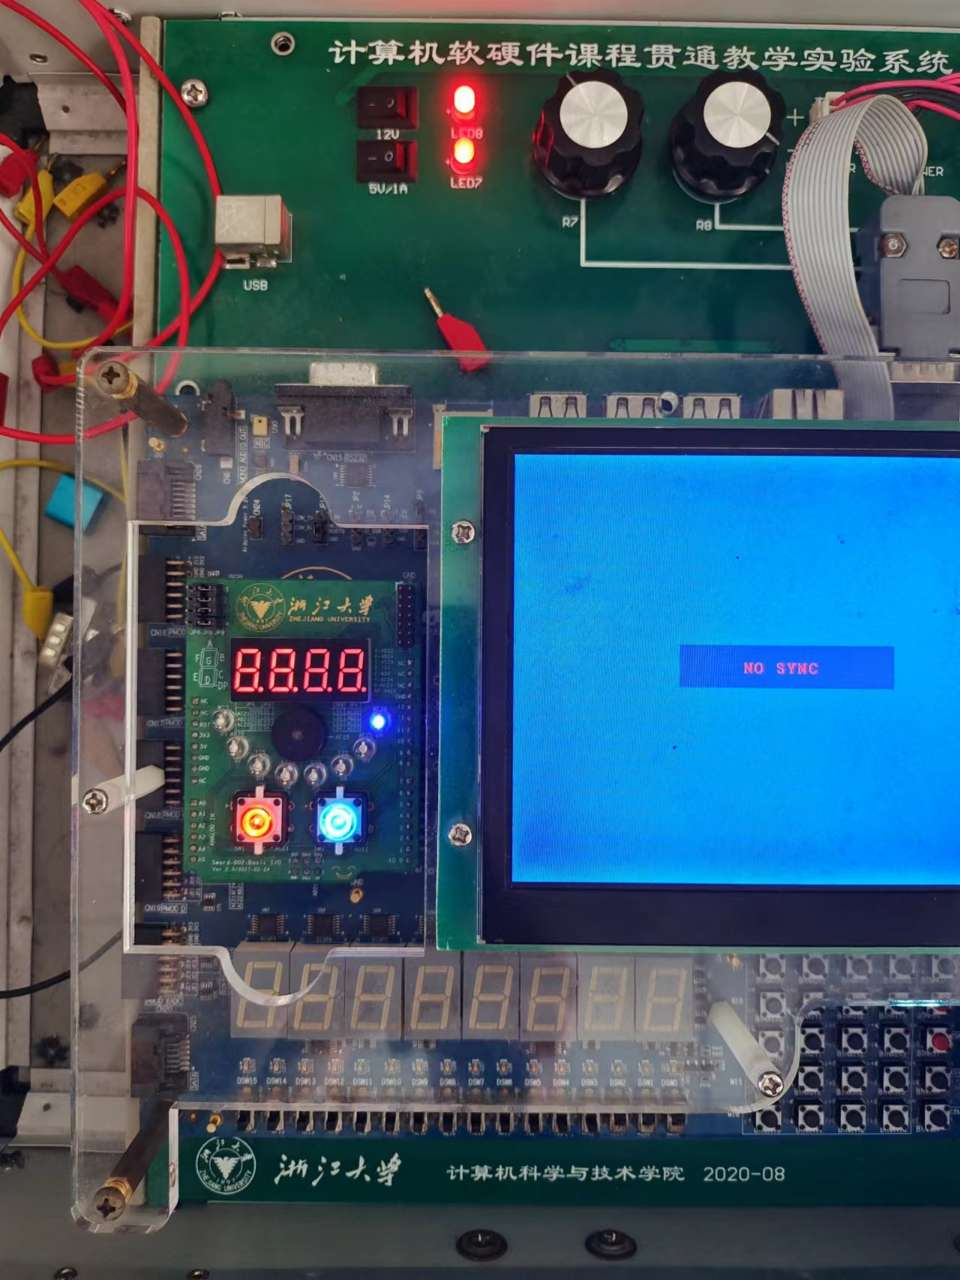
\includegraphics[width=0.4\textwidth]{21.jpg}
	\caption{\label{Lab5}下版验证}
	\end{figure}

	\begin{figure}[H]
	\centering
	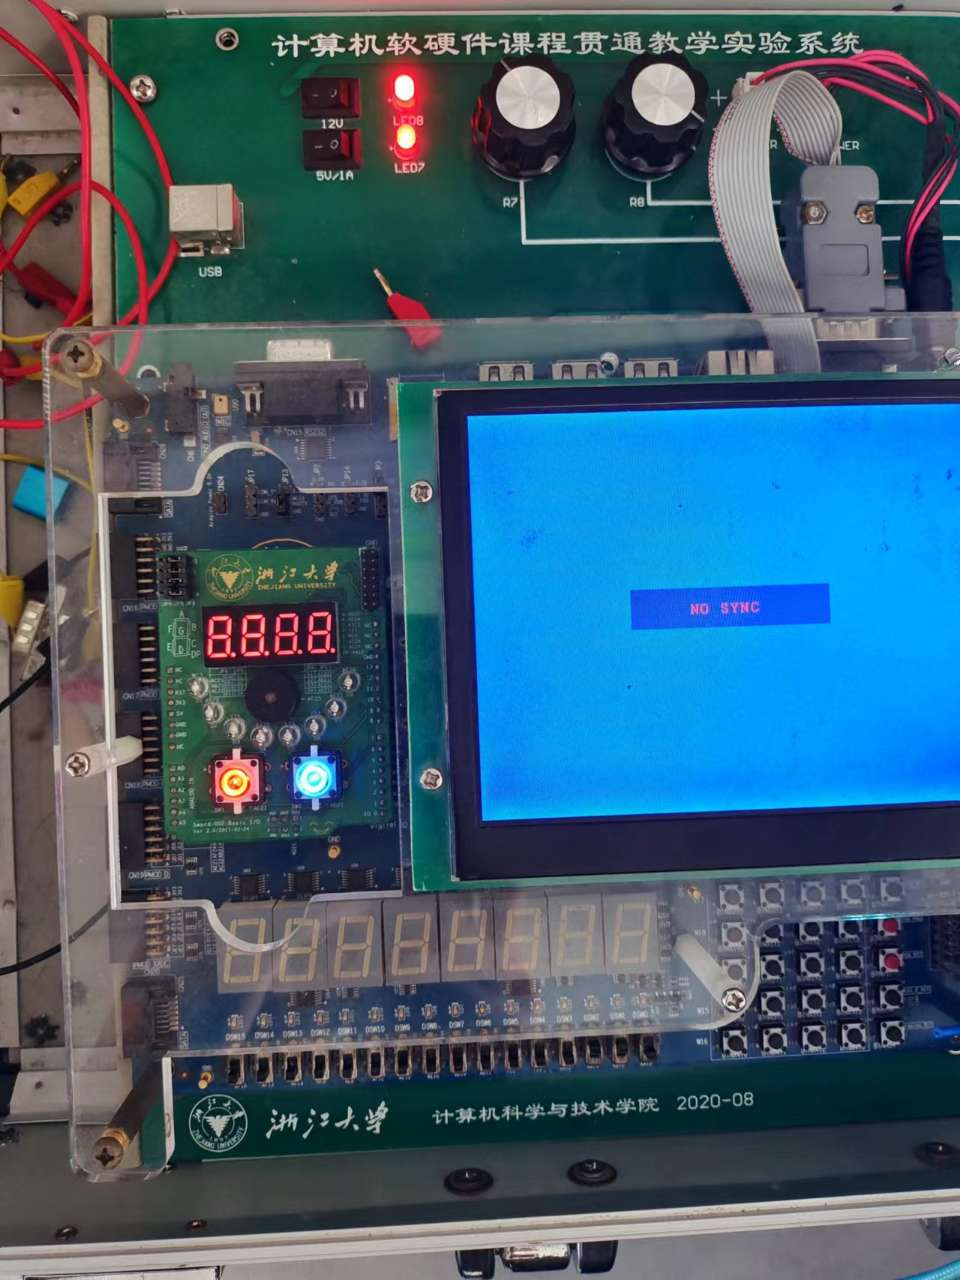
\includegraphics[width=0.4\textwidth]{22.jpg}
	\caption{\label{Lab5}下版验证}
	\end{figure}
\subsubsection*{下版现象解释:}
通过下版测试,当实验板被绑定的三个开关中,有奇数个开关被向上拨动时,可以看到,此时实验板所对应的灯会闪亮
如果被拨动的开关数目为偶数个,那么灯就不会闪亮,这与所实现的灯光控制的结构图是相符合的,当输入为\{1,1,1\},
\{1,0,0\},\{0,1,0\},\{0,0,1\}时,对应的输出F为1,因此,对应的灯会闪亮,这是与预期相符合的





\section{讨论与心得}
本次实验遇到的问题有:(1)用自己的电脑连接sword实验版时存在连接不上的问题,在更换了几个实验版后才找到可以连接的实验板.
(2)在实验时由于对应的引脚约束的顺序开始时有一定问题,导致下版的结果有一定的问题,在修改引脚约束之后才解决了问题.


\section{Bonous}
Bonous部分见1.4节

\end{document}